%    Documentation for Irrigation Control Project
%    Copyright (C) 2017  Gregory Raven
%
%    This program is free software: you can redistribute it and/or modify
%    it under the terms of the GNU General Public License as published by
%    the Free Software Foundation, either version 3 of the License, or
%    (at your option) any later version.
%
%    This program is distributed in the hope that it will be useful,
%    but WITHOUT ANY WARRANTY; without even the implied warranty of
%    MERCHANTABILITY or FITNESS FOR A PARTICULAR PURPOSE.  See the
%    GNU General Public License for more details.
%
%    You should have received a copy of the GNU General Public License
%    along with this program.  If not, see <http://www.gnu.org/licenses/>.

\chapter{Irrigation Scheduler Class}

The Scheduler class is responsible for activating the irrigation system at the 
time specified by the user.  The user enters the start and stop timing using 
the web browser controller.  The watering times are equally split between the 
two zones.

A timing function such as this might seem simple.  However, it proved 
challenging to implement with simple code.

Two excellent NPM packages came to the rescue: node-cron and moment.

\url{https://www.npmjs.com/package/moment}

The Node-cron package manager implements a functionality similar to a ``cron 
job'' in a POSIX operating system.  The function provided is a time-delayed 
task set by the user.  In this project, four jobs are required, and thus four 
node-cron tasks are created by a method of the Scheduler class.

The Moment package provides a robust data and time module which is more 
flexible than the native Javascript Date object.  The module's mode of 
operation is a little unusual, however, the documentation is excellent and the 
user should have no problem using the extensive feature set.

\url{https://www.npmjs.com/package/node-cron}

\begin{figure}[H]
	\centering
	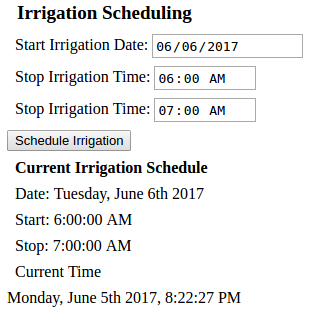
\includegraphics[width=0.6\textwidth]{photos/scheduler.png}
	\centering\bfseries
	\caption{The Web Browser Irrigation Scheduler}
\end{figure}

